\documentclass{article}

\usepackage{fancyhdr}
\usepackage{extramarks}
\usepackage{amsmath}
\usepackage{amsthm}
\usepackage{amsfonts}
\usepackage{tikz}
\usepackage[plain]{algorithm}
\usepackage{algpseudocode}
\usepackage{graphicx}
\usepackage{gensymb}
\usepackage{calc}
\usepackage[framed,numbered,autolinebreaks,useliterate]{mcode}
\usepackage{listings}

\graphicspath{{./images/}}

\usetikzlibrary{automata,positioning}

%
% Basic Document Settings
%

\topmargin=-0.45in
\evensidemargin=0in
\oddsidemargin=0in
\textwidth=6.5in
\textheight=9.0in
\headsep=0.25in

\linespread{1.1}

\pagestyle{fancy}
\lhead{\hmwkAuthorName}
\chead{\hmwkClass\ \hmwkTitle}
\rhead{\firstxmark}
\lfoot{\lastxmark}
\cfoot{\thepage}

\renewcommand\headrulewidth{0.4pt}
\renewcommand\footrulewidth{0.4pt}

\setlength\parindent{0pt}

%
% Create Problem Sections
%

\newcommand{\enterProblemHeader}[1]{
    \nobreak\extramarks{}{Problem {#1} continued on next page\ldots}\nobreak{}
    \nobreak\extramarks{{#1} (continued)}{{#1} continued on next page\ldots}\nobreak{}
}

\newcommand{\exitProblemHeader}[1]{
    \nobreak\extramarks{{#1} (continued)}{{#1} continued on next page\ldots}\nobreak{}
    % \stepcounter{#1}
    \nobreak\extramarks{{#1}}{}\nobreak{}
}

\setcounter{secnumdepth}{0}
\newcounter{partCounter}

\newcommand{\problemNumber}{0.0}

\newenvironment{homeworkProblem}[1][-1]{
    \renewcommand{\problemNumber}{{#1}}
    \section{\problemNumber}
    \setcounter{partCounter}{1}
    \enterProblemHeader{\problemNumber}
}{
    \exitProblemHeader{\problemNumber}
}

%
% Homework Details
%   - Title
%   - Class
%   - Author
%

\newcommand{\hmwkTitle}{Midterm}
\newcommand{\hmwkClass}{RBE 500}
\newcommand{\hmwkAuthorName}{\textbf{Arjan Gupta}}

%
% Title Page
%

\title{
    \vspace{2in}
    \textmd{\textbf{\hmwkClass\ \hmwkTitle}}\\
    \vspace{3in}
}

\author{\hmwkAuthorName}
\date{}

\renewcommand{\part}[1]{\textbf{\large Part \Alph{partCounter}}\stepcounter{partCounter}\\}

%
% Various Helper Commands
%

% Useful for algorithms
\newcommand{\alg}[1]{\textsc{\bfseries \footnotesize #1}}

% For derivatives
\newcommand{\deriv}[2]{\frac{\mathrm{d}}{\mathrm{d}#2} \left(#1\right)}

% For compact derivatives
\newcommand{\derivcomp}[2]{\frac{\mathrm{d}#1}{\mathrm{d}#2}}

% For partial derivatives
\newcommand{\pderiv}[2]{\frac{\partial}{\partial #2} \left(#1\right)}

% For compact partial derivatives
\newcommand{\pderivcomp}[2]{\frac{\partial #1}{\partial #2}}

% Integral dx
\newcommand{\dx}{\mathrm{d}x}

% Alias for the Solution section header
\newcommand{\solution}{\textbf{\large Solution}}

% Probability commands: Expectation, Variance, Covariance, Bias
\newcommand{\E}{\mathrm{E}}
\newcommand{\Var}{\mathrm{Var}}
\newcommand{\Cov}{\mathrm{Cov}}
\newcommand{\Bias}{\mathrm{Bias}}

\newlength\dlf% Define a new measure, dlf
\newcommand\alignedbox[2]{
% Argument #1 = before & if there were no box (lhs)
% Argument #2 = after & if there were no box (rhs)
&  % Alignment sign of the line
{
\settowidth\dlf{$\displaystyle #1$}  
    % The width of \dlf is the width of the lhs, with a displaystyle font
\addtolength\dlf{\fboxsep+\fboxrule}  
    % Add to it the distance to the box, and the width of the line of the box
\hspace{-\dlf}  
    % Move everything dlf units to the left, so that & #1 #2 is aligned under #1 & #2
\boxed{#1 #2}
    % Put a box around lhs and rhs
}
}

\begin{document}

\maketitle

\nobreak\extramarks{Problem 1}{}\nobreak{}

\pagebreak

\begin{homeworkProblem}[Problem 1]
    Derive the rotation matrix $R^1_2$ (you can leave sines and cosines as is).

    \begin{figure}[h]
        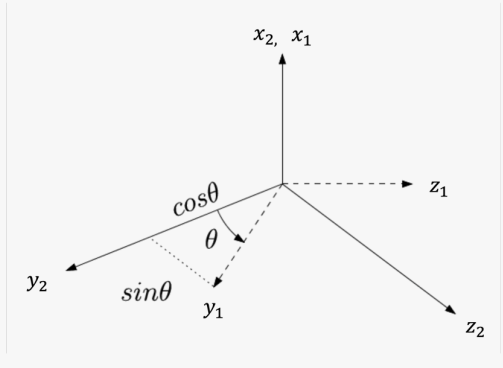
\includegraphics[scale=0.4]{q1_figure.png}
        \centering
    \end{figure}

    \subsection{Solution}

    Since the x-axis remains the same in the rotation, we know this is a basic 3D rotation matrix representing a rotation
    about the x-axis. However, using the right-hand screw rule, we see that the angle $\theta$ here is negative. So, by
    using equation (2.7) of our main textbook, the rotation matrix is given by,

    \begin{align*}
        &R^1_2 =
        \begin{bmatrix}
            1 & 0 & 0\\
            0 & \cos(-\theta) & -\sin(-\theta)\\
            0 & \sin(-\theta) & \cos(-\theta)\\
        \end{bmatrix}\\
        \alignedbox{}{R^1_2=
        \begin{bmatrix}
            1 & 0 & 0\\
            0 & \cos\theta & \sin\theta\\
            0 & -\sin\theta & \cos\theta\\
        \end{bmatrix}}
    \end{align*}
\end{homeworkProblem}

\nobreak\extramarks{Problem 2}{}\nobreak{}

\pagebreak

\begin{homeworkProblem}[Problem 2]
    Find the coordinates of point $p$ expressed in frame 1 (i.e. $p^1$) given the following.

    \[H^2_1 = \begin{bmatrix}
        1 & 0 & 0 & -1\\
        0 & 0.9553 & 0.2955 & -0.9553\\
        0 & -0.2955 & 0.9553 & 0.2955\\
        0 & 0 & 0 & 1
    \end{bmatrix},\text{   } p^2 = \begin{bmatrix}
        2\\
        5\\
        0
    \end{bmatrix}\]

    \subsection{Solution}

    From our knowledge of homogeneous transformations, we know that

    \[P^2 = H^2_1 P^1\]

    Where
    \(P^2 = \begin{bmatrix}
        p^2\\
        1
    \end{bmatrix}\) and \(P^1 = \begin{bmatrix}
        p^1\\
        1
    \end{bmatrix}\).\\

    However, we want to find

    We use the following MATLAB code for this computation.
\end{homeworkProblem}

\nobreak\extramarks{Problem 3}{}\nobreak{}

\pagebreak

\begin{homeworkProblem}[Problem 3]
    
\end{homeworkProblem}

\end{document}